\documentclass[accentcolor=tud1b,colorbacktitle,inverttitle,landscape,presentation,t]{tudbeamer}
\usepackage[utf8]{inputenc}
\usepackage[german]{babel}
\usepackage{verbatim, hyperref,multimedia}
\usepackage{graphicx, psfrag}			%to insert graphics
\usepackage{setspace}
\usepackage[active]{srcltx}
\usepackage{color}
\usepackage{subfigure}
\usepackage{listings}
\usepackage{pstricks}
\usepackage{amssymb}

\useinnertheme{default}
\usecolortheme{orchid}
\setbeamercovered{transparent}


\newcommand{\keyword}[1]{\textcolor{tudaccent}{\textbf{#1}}} 
\newcommand{\myframetitle}[2]{\frametitle{#1 \\[.2cm] \small #2}}
\newcommand{\fatitem}[1]{\item \textbf{#1}}
\newcommand{\tab}{\hspace*{0.5cm}}


\setcounter{tocdepth}{1} 

\hypersetup{
pdftitle={WebMining Exercise }, pdfauthor={F. Englert}
}


\begin{document}

\title[MGA]{\large 4. Exercise}

\author{Frank Englert, Jens Haase}
\institute{KE, TU Darmstadt}

\logo{
\includegraphics{graphics/keico.png}}

\date{Juni 2011}

\begin{titleframe}
\begin{center}
\color{tudtextaccent} \large Die 4. Übung\\[.5cm]
%\includegraphics[width=0.4\textwidth]{Graphics/spg_logo_final.eps} \\
\normalcolor \normalsize Knowlege Engineering \\
Fachbereich Informatik \\
Technische Universität Darmstadt\\[.5cm]

\textbf{Präsentation der Ergebnisse:}\\
Frank Englert\\ 
Jens Haase
\end{center}

\end{titleframe}  

\begin{frame}[c]
	\myframetitle{5. Übung}{Inhalt}
\begin{itemize}
  \fatitem{Sammeln der Daten}
  \fatitem{Page Rank und HITS}
  \begin{itemize}
  \item Implementierung von Page Rank
  \item Implementierung von HITS
  \item Vergleich der Ranking-Verfahren
  \item Berechnung der Kendall-Tau-Distanz
  \item Probleme des PageRank-Verfahrens
\end{itemize} 
\end{itemize} 
\end{frame}

\begin{frame}[c]
	\myframetitle{Task 1 - Language detection}{Language Detection via letter
	distribution}
\begin{itemize}
  \item The Firefox Plugin uses two detection modes
  \begin{itemize}
    \item Via letter frequency analysis
    \item Via syllable frequency analysis
  \end{itemize}
  \item The language detection algorithm is the same for both cases
  \item Advantages of using two detection modes:
  \begin{itemize}
    \item Double check the language detection results
    \item Collect information which mode works better
  \end{itemize}
  \item The Source of the frequency tables is http://bit.ly/jZHf0H
\end{itemize}
\end{frame}

\begin{frame}[c]
\myframetitle{Task 1 - Language detection}{Algorithm details}
\begin{itemize}
  \fatitem{The algorithms works with the following steps}
  \item A chunk is either a letter or a syllable
  \item dict contains the most important chunks of a language sorted by rank
\begin{enumerate}
  \item Take the text an split it to chunks(letters or syllables)
  \item Remove all chunks which are not in the dict
  \item Count the chunks and sort them by the count value. The result of this
  step is further called rankedChunks
  \item The weighted difference between the dictionary and the rankedChunks is
  \begin{itemize}
  \item $ \sum _{i=0}^{len(dic)} \frac{| i - rankedChunks.indexOf(dict[i]) |
  }{log _2 (i+2)}
  $
  \item If dict and rankedChunks are equals the weighted difference is 0
\end{itemize}
\end{enumerate}
\item repeat the steps 1-4 for all available languages. Take the language with
the lowest rank.
\end{itemize}
\end{frame}

\begin{frame}[c]
	\myframetitle{Task 1 - Language detection}{Letter frequency revisited}
\begin{figure}[htp]
\begin{center}
  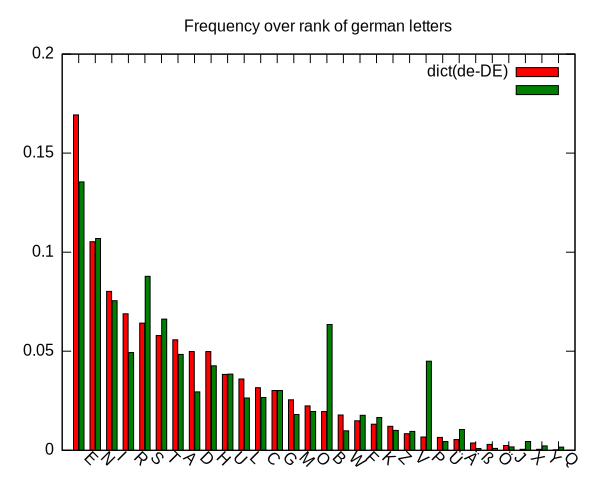
\includegraphics[width=1\textheight]{graphics/letters_de}
  \caption[fig:letters_de]{The frequency of german letters used
  for the Firefox plugin}
  \label{figureLabel}
\end{center}
\end{figure}

\end{frame}

\begin{frame}[c]
	\myframetitle{Task 1 - Language detection}{Syllable frequency revisited}

\begin{figure}[htp]
\begin{center}
  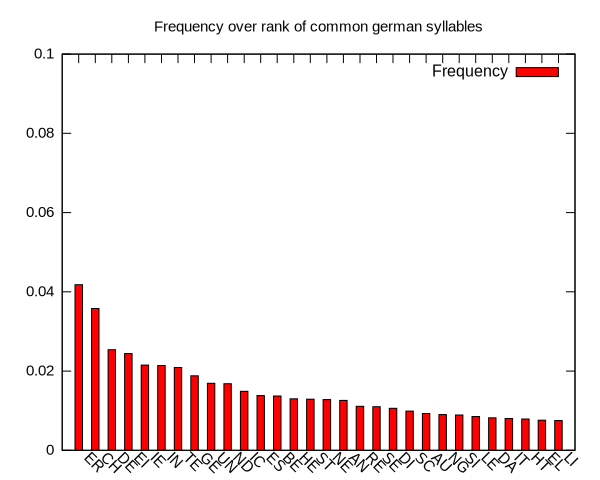
\includegraphics[width=1\textheight]{graphics/syllables_de}
  \caption[fig:letters_de]{The frequency of common german syllables used for the Firefox plugin}
  \label{figureLabel}
\end{center}
\end{figure}

\end{frame}


\begin{frame}[c]
	\myframetitle{Task 1 - Language detection}{Results of the language challenge}

\begin{table}
\begin{tabular}{|l|l|l|}
\hline
\textbf{Rank} &\textbf{letter lang}&\textbf{syllable lang}\\
\hline
1 &englisch&-\\
2 &englisch&-\\
3&deutsch&-\\
4&französisch&-\\
5&deutsch&-\\
6&deutsch&deutsch\\
7&französisch&französisch\\
8&französisch&französisch\\
9&englisch&englisch\\
10&deutsch&deutsch\\
\hline
\end{tabular}
\caption{Detection results of the firefox plugin}
\label{tablelabel}
\end{table}

\end{frame}

\begin{frame}[c]
	\myframetitle{Task 1 - Language detection}{Further improvement}
	
	\begin{itemize}
	\fatitem{Easy:}
	\begin{itemize}
		\item Add more languages
	\end{itemize}
	
	  \fatitem{A lot of work:}
	  \begin{itemize}
  	    \item The Plugin checks already p, div and span tags. It would be better
  	  to check the text content of all tags.
  	    \item Try to estimate the best detection result if the syllable and the
  	letter mode returns different results
      \end{itemize}
      \fatitem{Most Interesting:}
      \begin{itemize}
  		\item Improve the weighting algorithm to reduce the amount of needed text
  		\item Implement a learning mode to train new languages

	\end{itemize}
	\end{itemize}
\end{frame}
\begin{frame}[c]
  \myframetitle{Aufgabe 2}{Suche mittels HITS}
\begin{itemize}
  \item Berechnet die Wahrscheinlichkeit das eine Seite ein Hub oder eine Authority ist
  \item Muss bei jeder Suchanfrage neu berechnet werden
  \item In der Übung wurde die Iterative Methode verwendet
  \item Der Algorithmus terminiert meistens nach 11 Iterationen
\end{itemize}
\end{frame}

\begin{frame}[c]
    \myframetitle{HITS}{Authority ist hoch bei vielen eingehenden Links}
    %\usepackage{graphics} is needed for \includegraphics
\begin{figure}[htp]
\begin{center}
  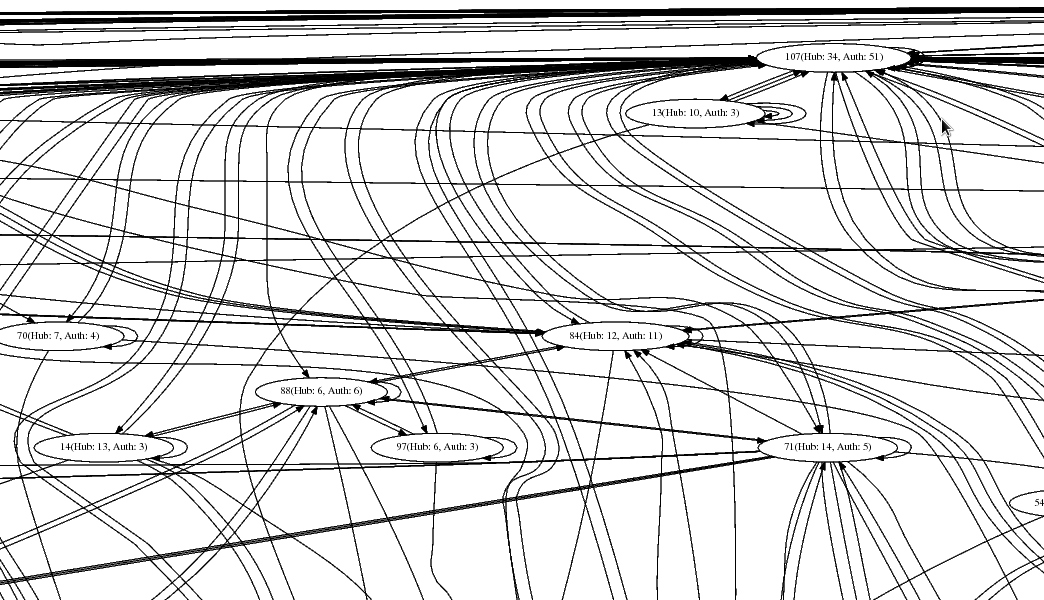
\includegraphics[height=1\textheight]{graphics/hitsGraph.png}
%  \caption[labelInTOC]{}
%  \label{fig:hihg_inoutdegree}
\end{center}
\end{figure}

\end{frame}
\begin{frame}[c]
  \myframetitle{Aufgabe 2}{Suche mittels Page-Rank}
\begin{itemize}
  \fatitem{Der Page-Rank ist die Wahrscheinlichkeit eines Websiten-Besuchs}
  \item Das Ranking der Websites kann offline erfolgen
  \item Für die Übung wurde das Iterative Pagerank-Verfahren implementiert
  \item Der Algorithmus konvergiert nach 30 Iterationen auf dem Beispielgraph
\end{itemize}
\end{frame}

\begin{frame}[c]
\myframetitle{Page-Rank}{Verteilung des Page-Ranks}
%\usepackage{graphics} is needed for \includegraphics
\begin{figure}[htp]
\begin{center}
  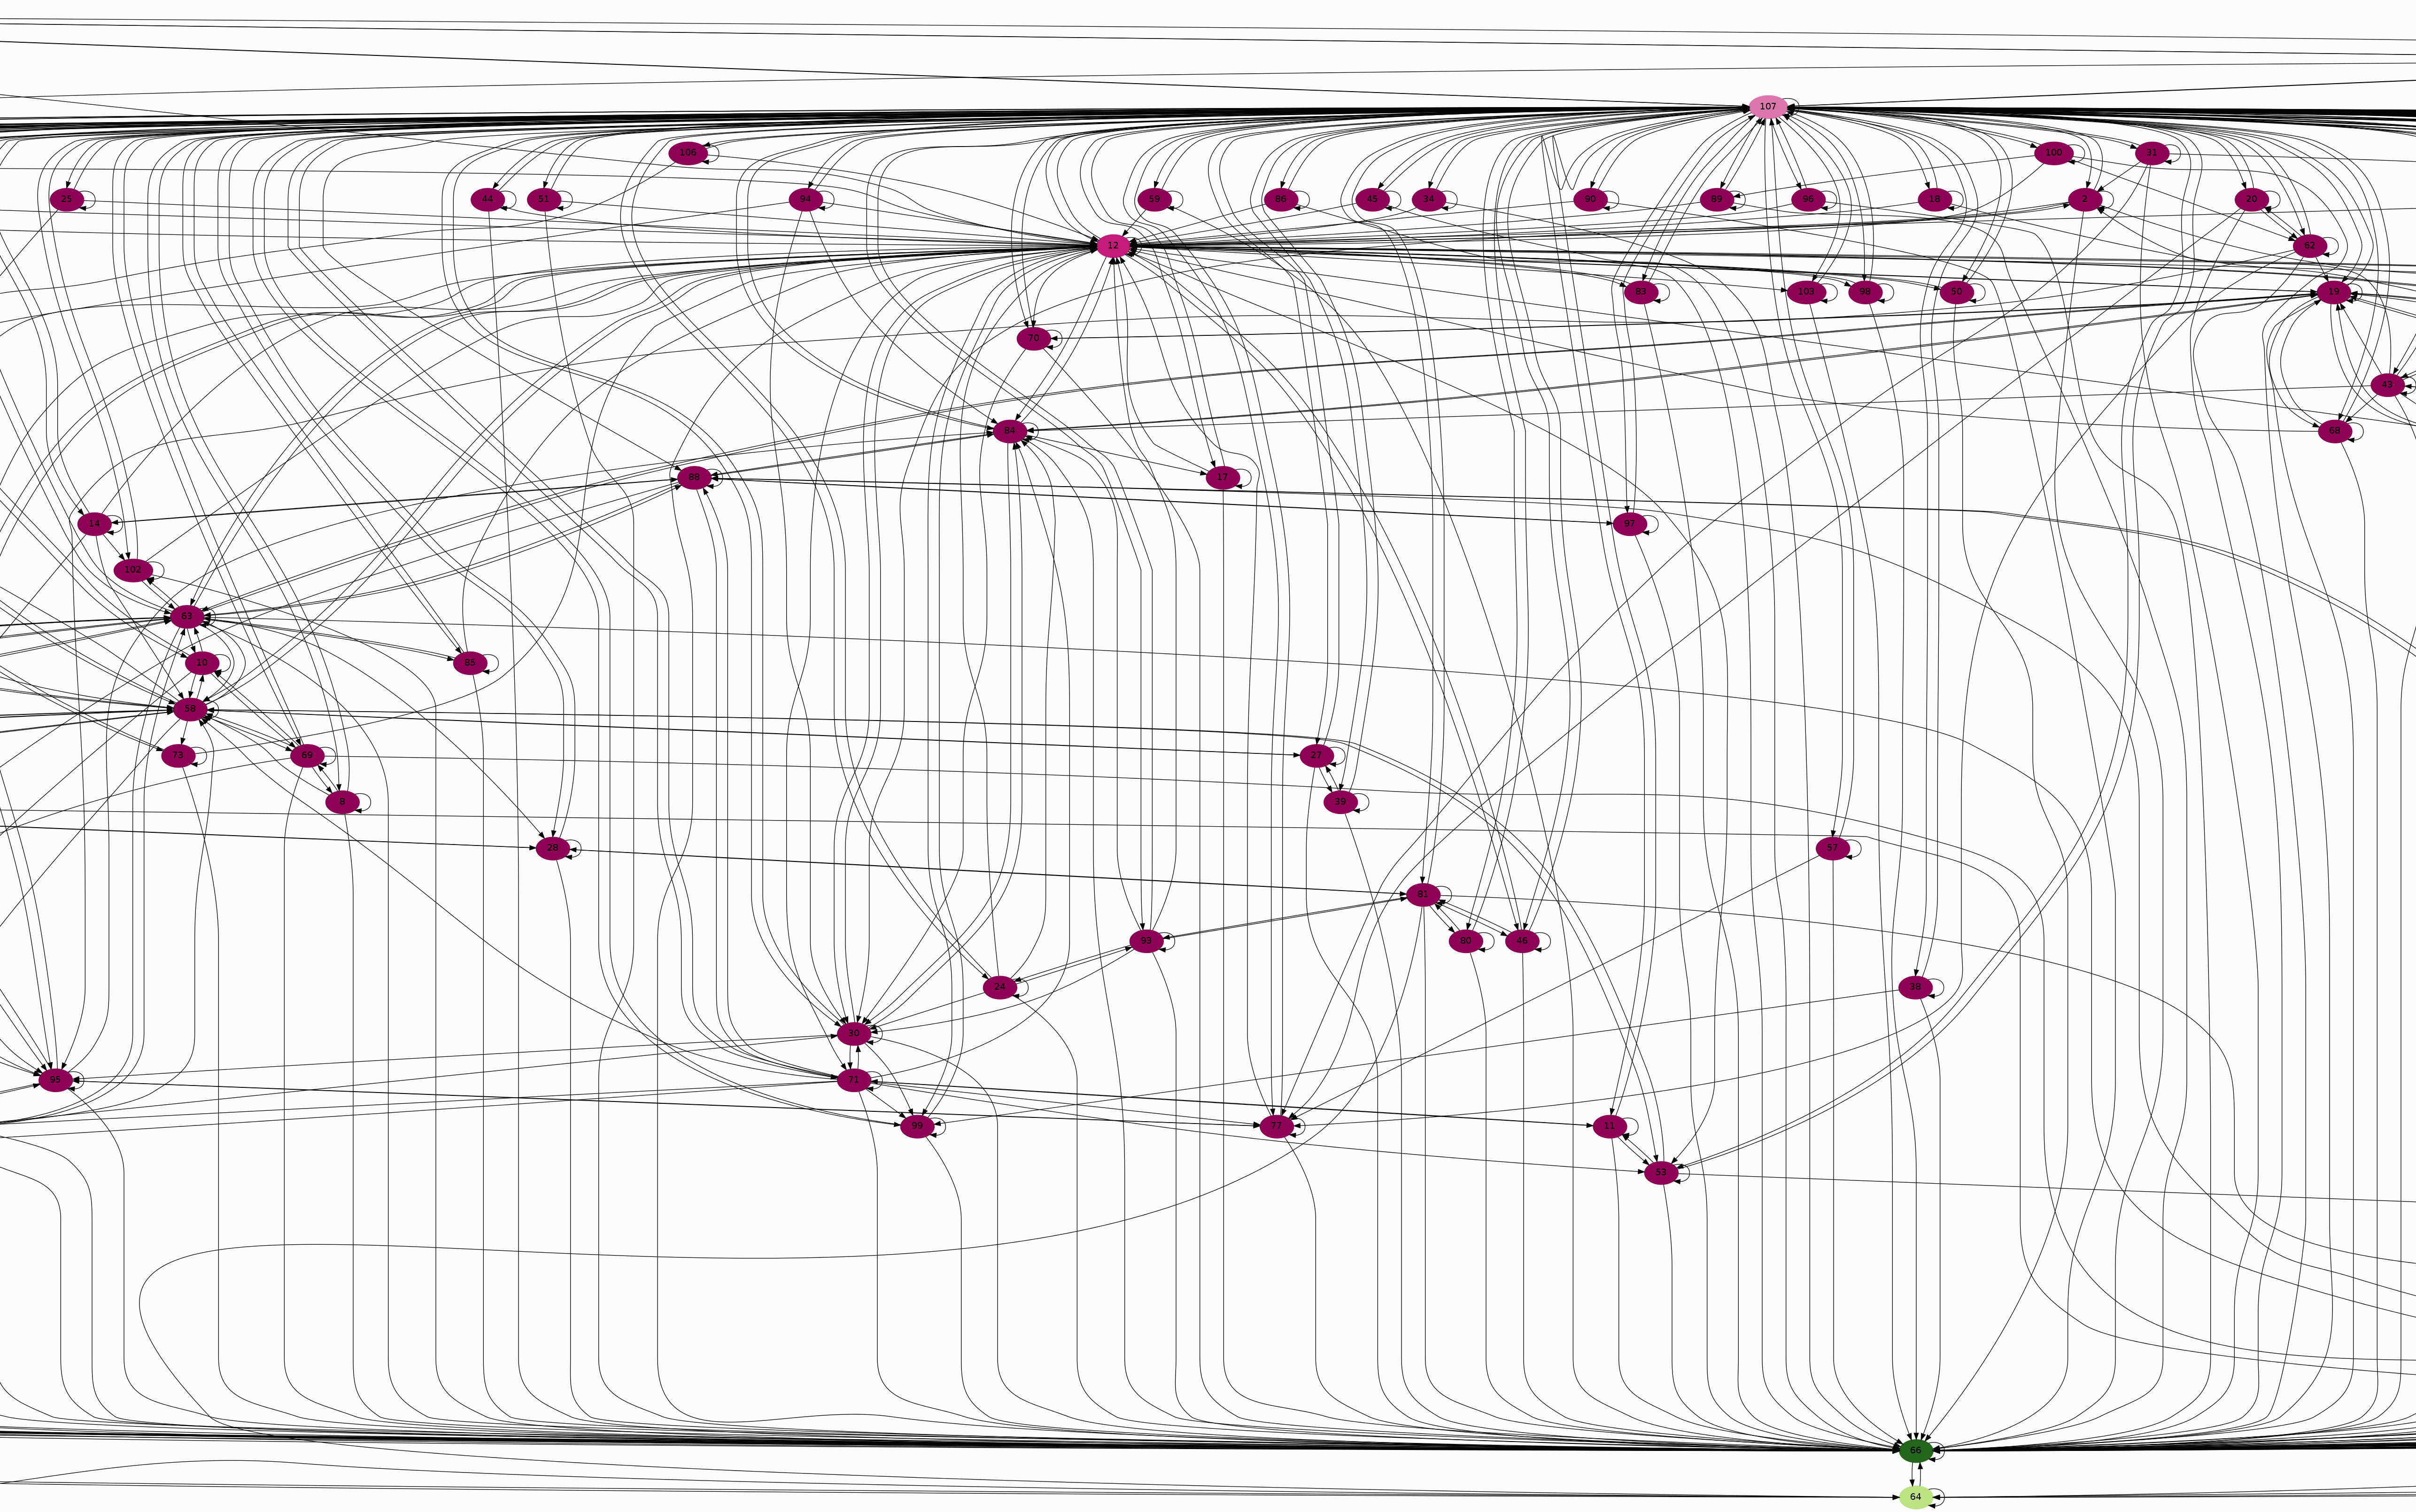
\includegraphics[height=1\textheight]{graphics/pr_overview.png}
  \caption[labelInTOC]{}
  \label{fig:prOverview} 
\end{center}
\end{figure}
\end{frame}

\begin{frame}[c]
    \myframetitle{Page-Rank}{PR ist hoch bei hohem In-Degree}
    %\usepackage{graphics} is needed for \includegraphics
\begin{figure}[htp]
\begin{center}
  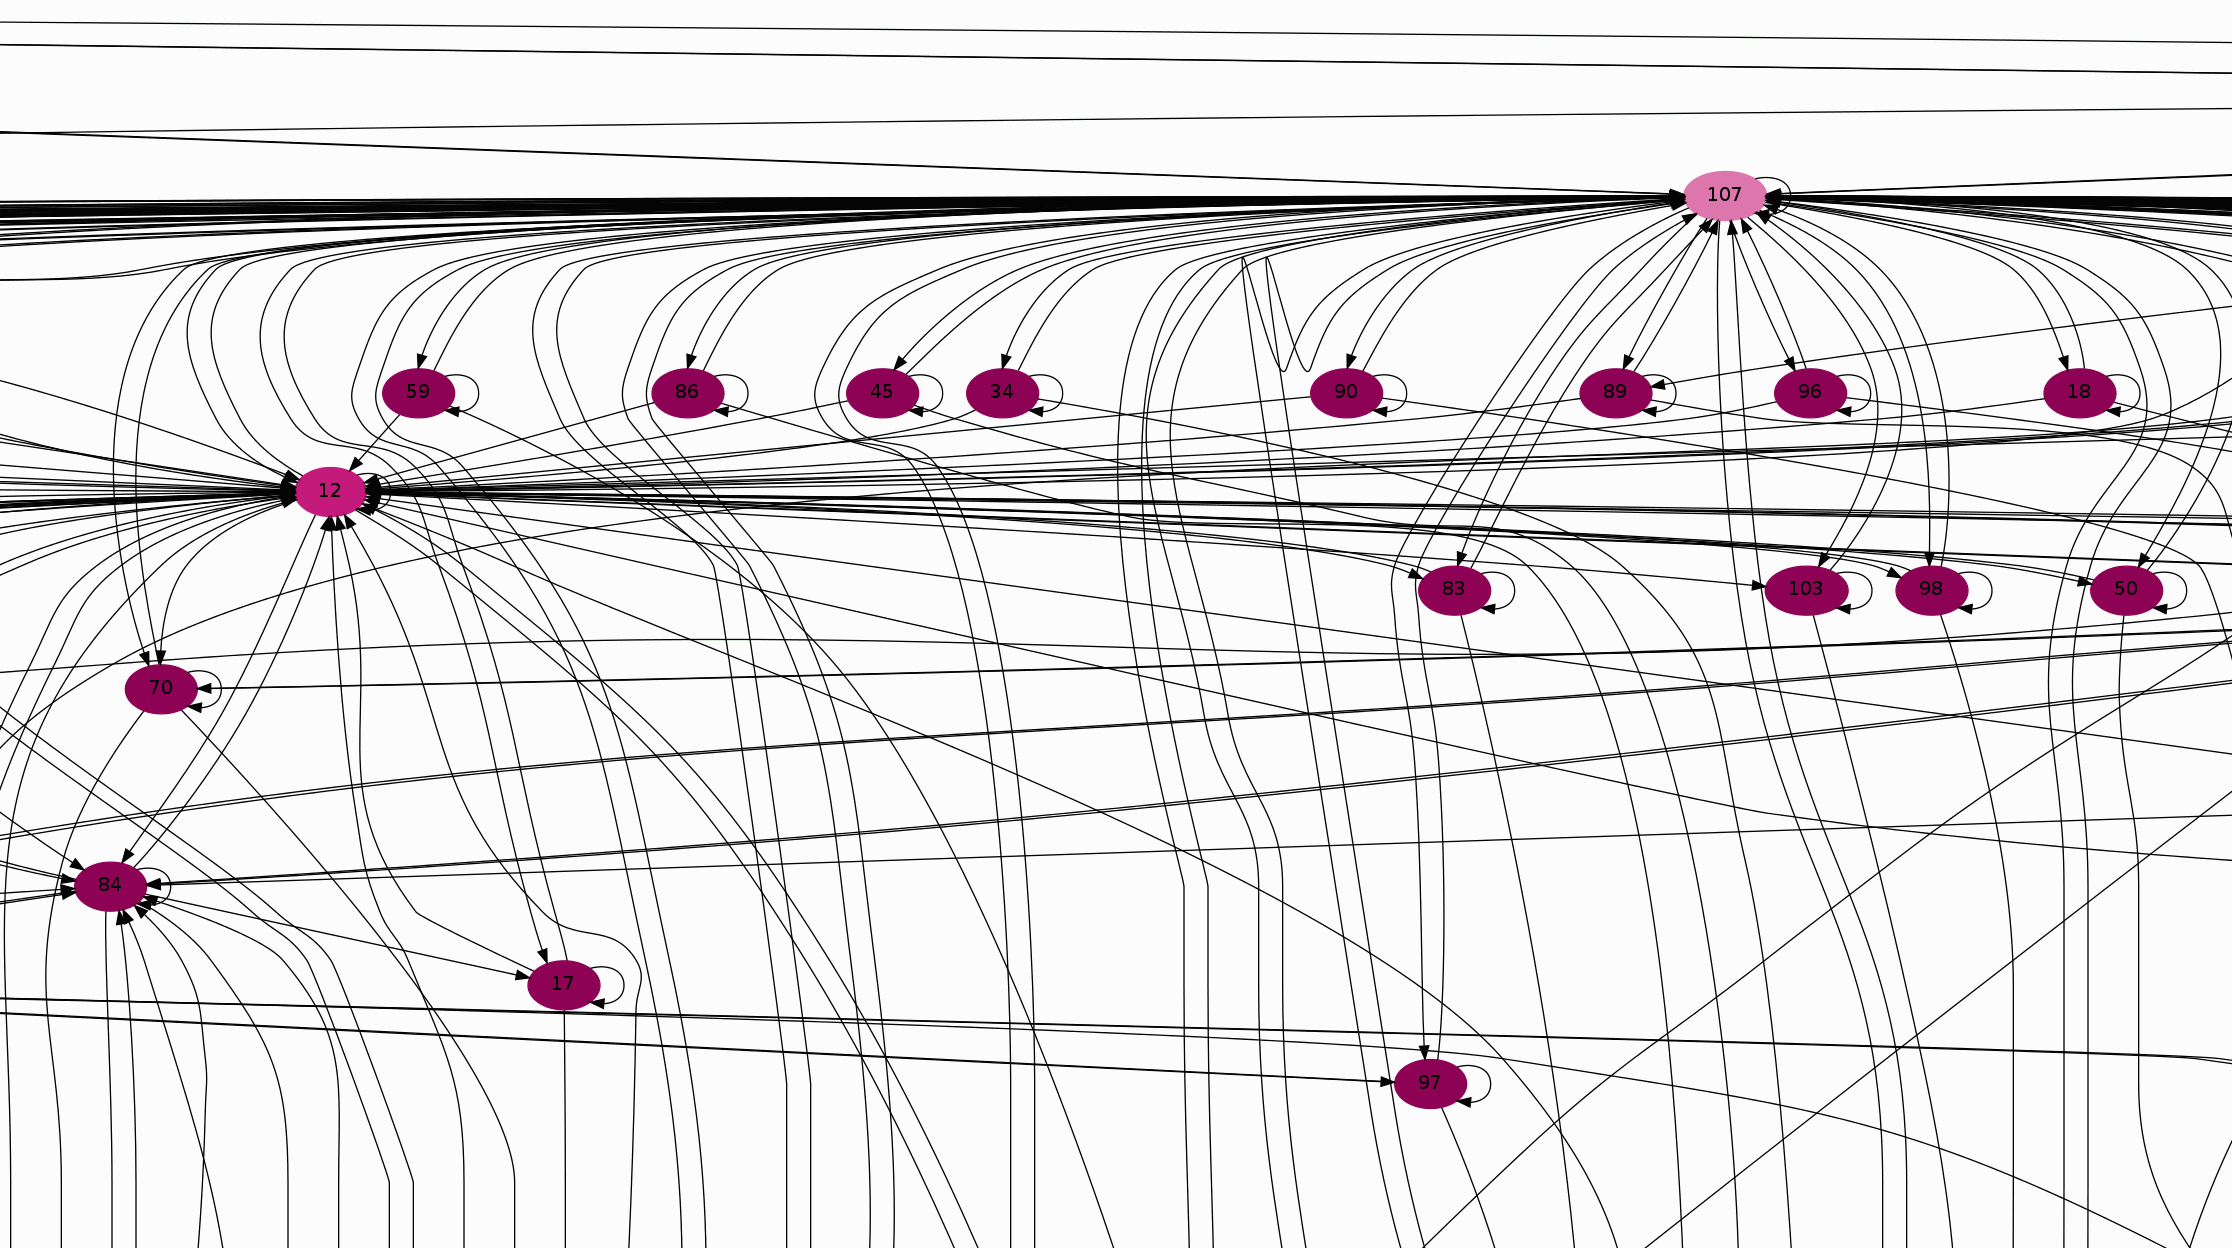
\includegraphics[height=1\textheight]{graphics/pr_high_inout_degree.png}
%  \caption[labelInTOC]{}
%  \label{fig:hihg_inoutdegree}
\end{center}
\end{figure}

\end{frame}


\begin{frame}[c]
    \myframetitle{Page-Rank}{PR ist hoch bei kleinem Out-Degree der Vorgänger}
%\usepackage{graphics} is needed for \includegraphics
\begin{figure}[htp]
\begin{center}
  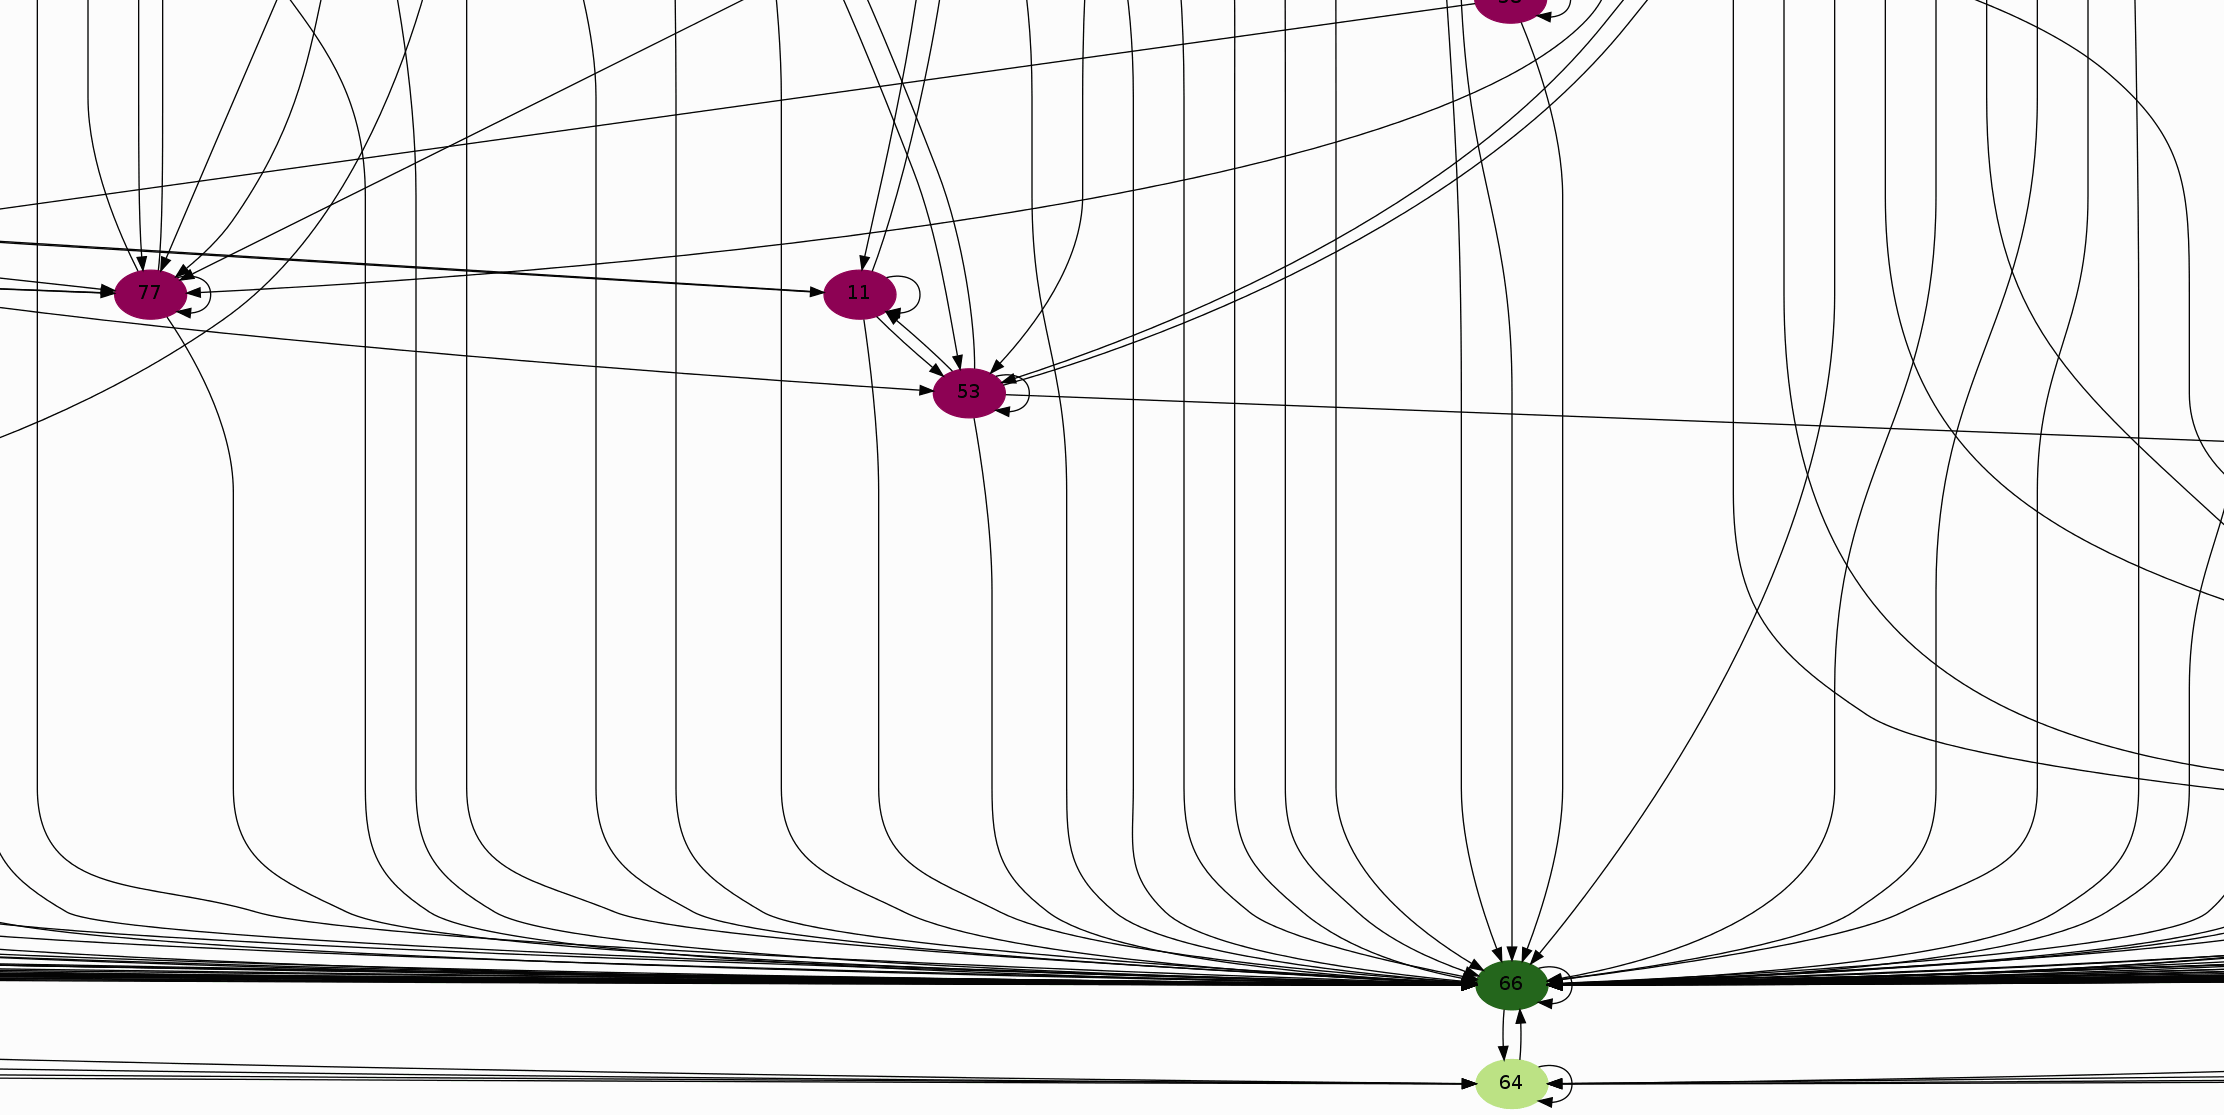
\includegraphics[height=1\textheight]{graphics/high_indegree.png}
%  \caption[labelInTOC]{}
%  \label{fig:prHighIndegree}
\end{center}
\end{figure}
\end{frame}

\begin{frame}[c]
    \myframetitle{Page-Rank}{Ranking des Graphen aus Aufgabe 1}
    \begin{itemize}
  \fatitem{Für den Graph aus Aufgabe 1 ergibt sich folgendes Ranking:}
\begin{enumerate}
  \item ID(66)	PR(0,28804), Special Categories
  \item ID(64)	PR(0,22126), Wikipedia Categorization
  \item ID(107) PR(0,06453), Category Data mining
  \item ID(12)	PR(0,03134), Data mining
  \item ID(91)	PR(0,01396), Why  might a category list\ldots
  \item ID(58)	PR(0,01061), Cluster analysis
\end{enumerate}
\ldots
\begin{enumerate}[100.]
\item  ID(104)	PR(0,00223), Affinity analysis
\end{enumerate}
\item Max(PR)=0,28804 Min(PR)=0.00223
\item Die Wahrscheinlichkeit durch zufälliges Surfen auf die Seite
``Special Categories'' zu kommen beträgt demnach 28\%
\item Die Wahrscheinlichkeit durch zufälliges Surfen auf ``Affinity Analysis'' zu
kommen beträgt nur 0.2\%
\end{itemize}
\end{frame}


% I: Query is:machine + learning
% I: Found 28 hits.
% I: #107	PR(0,06453), http://en.wikipedia.org/wiki/Category:Data_mining
% I: #12	PR(0,03134), http://en.wikipedia.org/wiki/Data_mining
% I: #58	PR(0,01061), http://en.wikipedia.org/wiki/Cluster_analysis
% I: #19	PR(0,0093), http://en.wikipedia.org/wiki/Text_mining
% I: #84	PR(0,00879), http://en.wikipedia.org/wiki/RapidMiner
% I: #95	PR(0,00813), http://en.wikipedia.org/wiki/Association_rule_learning
% I: #30	PR(0,00807), http://en.wikipedia.org/wiki/Weka_(machine_learning)
% I: #99	PR(0,00625), http://en.wikipedia.org/wiki/Receiver_operating_characteristic
% I: #60	PR(0,00578), http://en.wikipedia.org/wiki/Correlation_clustering
% I: #33	PR(0,00553), http://en.wikipedia.org/wiki/Overfitting
% I: #21	PR(0,00549), http://en.wikipedia.org/wiki/Neural_network
% I: #9	PR(0,00513), http://en.wikipedia.org/wiki/Formal_concept_analysis
% I: #2	PR(0,00438), http://en.wikipedia.org/wiki/Decision_tree_learning
% I: #46	PR(0,00437), http://en.wikipedia.org/wiki/Reactive_Business_Intelligence
% I: #75	PR(0,00433), http://en.wikipedia.org/wiki/Principal_component_analysis
% I: #98	PR(0,00404), http://en.wikipedia.org/wiki/Profiling_practices
% I: #26	PR(0,0035), http://en.wikipedia.org/wiki/K-optimal_pattern_discovery
% I: #68	PR(0,00348), http://en.wikipedia.org/wiki/Web_mining
% I: #73	PR(0,00319), http://en.wikipedia.org/wiki/Consensus_clustering
% I: #80	PR(0,003), http://en.wikipedia.org/wiki/DataRush_Technology
% I: #93	PR(0,00299), http://en.wikipedia.org/wiki/Data_stream_mining
% I: #6	PR(0,0029), http://en.wikipedia.org/wiki/Elastic_map
% I: #89	PR(0,00283), http://en.wikipedia.org/wiki/Molecule_mining
% I: #24	PR(0,00254), http://en.wikipedia.org/wiki/Concept_drift
% I: #106	PR(0,00243), http://en.wikipedia.org/wiki/Zementis_Inc
% I: #34	PR(0,00243), http://en.wikipedia.org/wiki/Data_mining_in_meteorology
% I: #94	PR(0,00223), http://en.wikipedia.org/wiki/Feature_Selection_Toolbox
% I: #31	PR(0,00223), http://en.wikipedia.org/wiki/List_of_machine_learning_algorithms

\begin{frame}[c]
    \myframetitle{2.2 Vergleich der Verfahren}{Mit dem Query ``Machine Learning''}
\begin{table}
\begin{tabular}{r|r|r|r}
\textbf{Page Rank} & \textbf{Hub} & \textbf{Auth} \\
\hline
107 (0,06453) & 107 (0.33741316) & 107 (0.51394016) \\
12 (0,03134)  & 12 (0.21790208)  & 12 (0.4670657) \\
58 (0,01061)  & 2 (0.202119)     & 58 (0.17513451) \\
19 (0,0093)   & 58 (0.18476191)  & 30 (0.14663029) \\
84 (0,00879)  & 19 (0.16472404)  & 84 (0.11436833) \\
95 (0,00813)  & 94 (0.14808507)  & 19 (0.107671805) \\
30 (0,00807)  & 84 (0.12306109)  & 95 (0.08477965) \\
99 (0,00625)  & 75 (0.12220599)  & 53 (0.07186372) \\
60 (0,00578)  & 46 (0.115581095) & 2 (0.06686905) \\
\end{tabular}
\caption{Vergleich des Page-Rank mit den Ergebnissen des HITS sortiert nach jeweiligem Ranking.}
\label{tbl:pr_vs_hits}
\end{table}

\end{frame}
% 
% I: Query is:web + mining
% I: Found 15 hits.
% I: #12	PR(0,03134), http://en.wikipedia.org/wiki/Data_mining
% I: #58	PR(0,01061), http://en.wikipedia.org/wiki/Cluster_analysis
% I: #19	PR(0,0093), http://en.wikipedia.org/wiki/Text_mining
% I: #84	PR(0,00879), http://en.wikipedia.org/wiki/RapidMiner
% I: #68	PR(0,00348), http://en.wikipedia.org/wiki/Web_mining
% I: #48	PR(0,00317), http://en.wikipedia.org/wiki/Biomedical_text_mining
% I: #93	PR(0,00299), http://en.wikipedia.org/wiki/Data_stream_mining
% I: #5	PR(0,00286), http://en.wikipedia.org/wiki/Co-occurrence_networks
% I: #15	PR(0,00267), http://en.wikipedia.org/wiki/Deep_Web_Technologies
% I: #105	PR(0,00267), http://en.wikipedia.org/wiki/Ren-rou
% I: #106	PR(0,00243), http://en.wikipedia.org/wiki/Zementis_Inc
% I: #90	PR(0,00243), http://en.wikipedia.org/wiki/Software_mining
% I: #45	PR(0,00243), http://en.wikipedia.org/wiki/Able_Danger
% I: #82	PR(0,00231), http://en.wikipedia.org/wiki/Data_mining_in_agriculture
% I: #78	PR(0,00231), http://en.wikipedia.org/wiki/KXEN_Inc.
% D: Done

\begin{frame}[c]
    \myframetitle{2.3 Ausgabe der PageRank-Suche}{Für die Query ``web mining''}

\begin{table}
\begin{tabular}{r|r|r|r}
	 & \textbf{Page Rank} & \textbf{Hub} & \textbf{Auth} \\
	\hline
	Recall 				&  & 0.583 & 0.583 \\
	Precision 			&  & 0.146 & 0.146 \\
	Average Precision 	&  & 0.39  & 0.39  \\
	NDCG 				&  & 0.586 & 0.586 \\
	Kendall tau 		&  & 0.429 & 0.381 \\
\end{tabular}
\caption{Vergleich Page Rank und HITS}
\end{table}

\end{frame}
% 
% I: Query is:web + mining
% I: Found 15 hits.
% I: #12	PR(0,03134), http://en.wikipedia.org/wiki/Data_mining
% I: #58	PR(0,01061), http://en.wikipedia.org/wiki/Cluster_analysis
% I: #19	PR(0,0093), http://en.wikipedia.org/wiki/Text_mining
% I: #84	PR(0,00879), http://en.wikipedia.org/wiki/RapidMiner
% I: #68	PR(0,00348), http://en.wikipedia.org/wiki/Web_mining
% I: #48	PR(0,00317), http://en.wikipedia.org/wiki/Biomedical_text_mining
% I: #93	PR(0,00299), http://en.wikipedia.org/wiki/Data_stream_mining
% I: #5	PR(0,00286), http://en.wikipedia.org/wiki/Co-occurrence_networks
% I: #15	PR(0,00267), http://en.wikipedia.org/wiki/Deep_Web_Technologies
% I: #105	PR(0,00267), http://en.wikipedia.org/wiki/Ren-rou
% I: #106	PR(0,00243), http://en.wikipedia.org/wiki/Zementis_Inc
% I: #90	PR(0,00243), http://en.wikipedia.org/wiki/Software_mining
% I: #45	PR(0,00243), http://en.wikipedia.org/wiki/Able_Danger
% I: #82	PR(0,00231), http://en.wikipedia.org/wiki/Data_mining_in_agriculture
% I: #78	PR(0,00231), http://en.wikipedia.org/wiki/KXEN_Inc.
% D: Done

\begin{frame}[c]
    \myframetitle{2.4 Recall, Precision, NDCG}{Für die Query ``web mining''}

\begin{table}
\begin{tabular}{r|r|r|r|r}
	 & \textbf{Wahres Ranking }& \textbf{Page Rank} & \textbf{Hub} & \textbf{Auth}
	 \\
	\hline
	Recall 				& 1.00 	& 0.500 & 0.583 & 0.583 \\
	Precision 			& 1.00 	& 0.500 & 0.146 & 0.146 \\
	Average Precision 	& 1.00 	& 0.409 & 0.39  & 0.39  \\
	NDCG 				& 1.00 	& 0.591 & 0.586 & 0.586 \\
	Kendall tau 		& 0		& 0.333 & 0.429 & 0.381 \\
\end{tabular}
\caption{Vergleich Page Rank und HITS}
\end{table}

\end{frame}
\begin{frame}[c]
  \myframetitle{Ranking-Verfahren}{Im Vergleich}

  \begin{itemize}
  \fatitem{Alle Ranking-Verfahren eignen sich für einen Vergleich der
  Suchergebnisse}
  \item Das tatsächlich beste Verfahren muss Anhand der Anforderungen gewählt
  werden
  \item Jen nach dem, auf welche Anforderungen die Suchmaschine optimiert werden
  soll, eignen sich die Ranking-Verfahren unterschiedlich gut.
  \begin{itemize}
    \item \textit{Precision} und \textit{Recall} ermöglichen ein Optimieren der
    Suchmaschine auf False-Positive und False-Negative-Fehlerraten. Die Qualität
    des Rankings kann nicht gemessen werden
    \item \textit{NDCG} ermöglicht ein Optimieren der Suchmaschine falls nur
    wenige Suchergebnisse gewünscht sind. Je höher der Rang, desto geringer ist der
    Einfluss eines Ergebnisdokuemnts auf das Messergebniss
    \item Die \textit{Kendall-Tau-Distanz} ermöglicht das Bestimmen der Güte
    der Sortierung der Ebnissdokumente. Es werden dabei aber keinerlei Aussagen
    über die Fehlerrate getroffen
  \end{itemize}
\end{itemize}
\end{frame}

\begin{frame}[c]
  \myframetitle{Suchverfahren im Vergleich}{HITs vs. Page-Rank}
  \begin{itemize}
  \item HITs hat einen höheren Recall bei einer geringeren Precision
  $\rightarrow$ HITs liefert mehr Ergebnisdokumente zurück.
\item   Die \textit{normalized discountent cumulative Gain} und
\textit{average Precision} haben ähnliche Werte. 
  \item Allerdings ist die \textit{normalisierte Kendall-Tau-Distanz} des
  HITs-Ergebnissets höher. Das bedeutet, PageRank sortiert die Ergebnisse
  besser.
  \fatitem{$\Rightarrow$ HITs liefert mehr gewünschte Ergebnisse während bei
  Page-Rank die Sortierung der Ergebnisse besser ist}
\end{itemize}

  
\end{frame}
\begin{frame}[c]
  \myframetitle{2.6 Probleme des Page-Ranks}{Und Lösungmöglichkeiten}

  \begin{itemize}
  \item \textbf{Problem:} Page-Rank zeigt bei vielen Abfagen Data-Mining als
  wichtigstes Dokument an
  \item $\rightarrow$ dies passiert, weil von vielen Seiten auf ``Data-Mining''
  verlinkt wird.
  \fatitem{Es darf nicht allein der Page-Rank zur Sortierung der Suchergebnisse
  verwendet werden}
  \item Es müssen weitere Informationen verwendet werden, um die
  Sortierreihenfolge der Ergebnisse zu bestimmen
  \begin{itemize}
  \item Beispielsweise ob der Query auf den Seitentitel oder eine Überschrift
  trifft
  \item Ob Benuzter das Suchergebnis empfehlen können
  \item Allerdings ist das Gewichten der Suchergebnisse laut Script eine
  ``schwarze Kunst'' :-)
\end{itemize}
\end{itemize}
\end{frame}
\end{document}
